Epitaxy has been a dominant technological feature since near the inception of the semiconductor age.
It has also been intimately entwined with the dominant semiconductor up till the present day, silicon.
Silicon has been a dominant player in almost every field of semiconductor research for the better part of 40 years, becoming the most well understood material in the world.
This focus on silicon has also greatly influenced the thinking of what were at the time fledgling fields, most notably epitaxy.
\emph{Epi-taxis} or ``above --- in an ordered manner'' is the Greek root of the term epitaxy and as it is originally defined, it has been narrowly interpreted by most of the research field.
Silicon on silicon epitaxy, or homoepitaxy, has been the dominant type of epitaxy both for research and production, due to its relevance to semiconductor chip manufacturing.
This idea of the `ideal' epitaxy as modelled by silicon homoepitaxy has pervaded the thinking of research into the field, with the material systems being most similar as the result being the most researched, and the most successful.

The material systems most similar to homoeptiaxy (besides other homoepitaxy) are the III-V group semiconductors, specifically the Al/Ga/In-P/As/Sb bi\-nary/ter\-nary/qua\-ter\-nary family as in \cref{fig:intro_bandgaps}.
These zincblende semiconductors through the manipulation of exact atomic concentration, can be grown from exactly lattice matched to strongly mismatched.
These material systems all have covalent or primarily covalent bonds with strongly preferred atomic sites for the atomic species.
When parameters are optimized, epitaxial growth in such systems is orientationally commensurate with the underlying substrate and dominated by strain effects.
\begin{figure}
 \centering 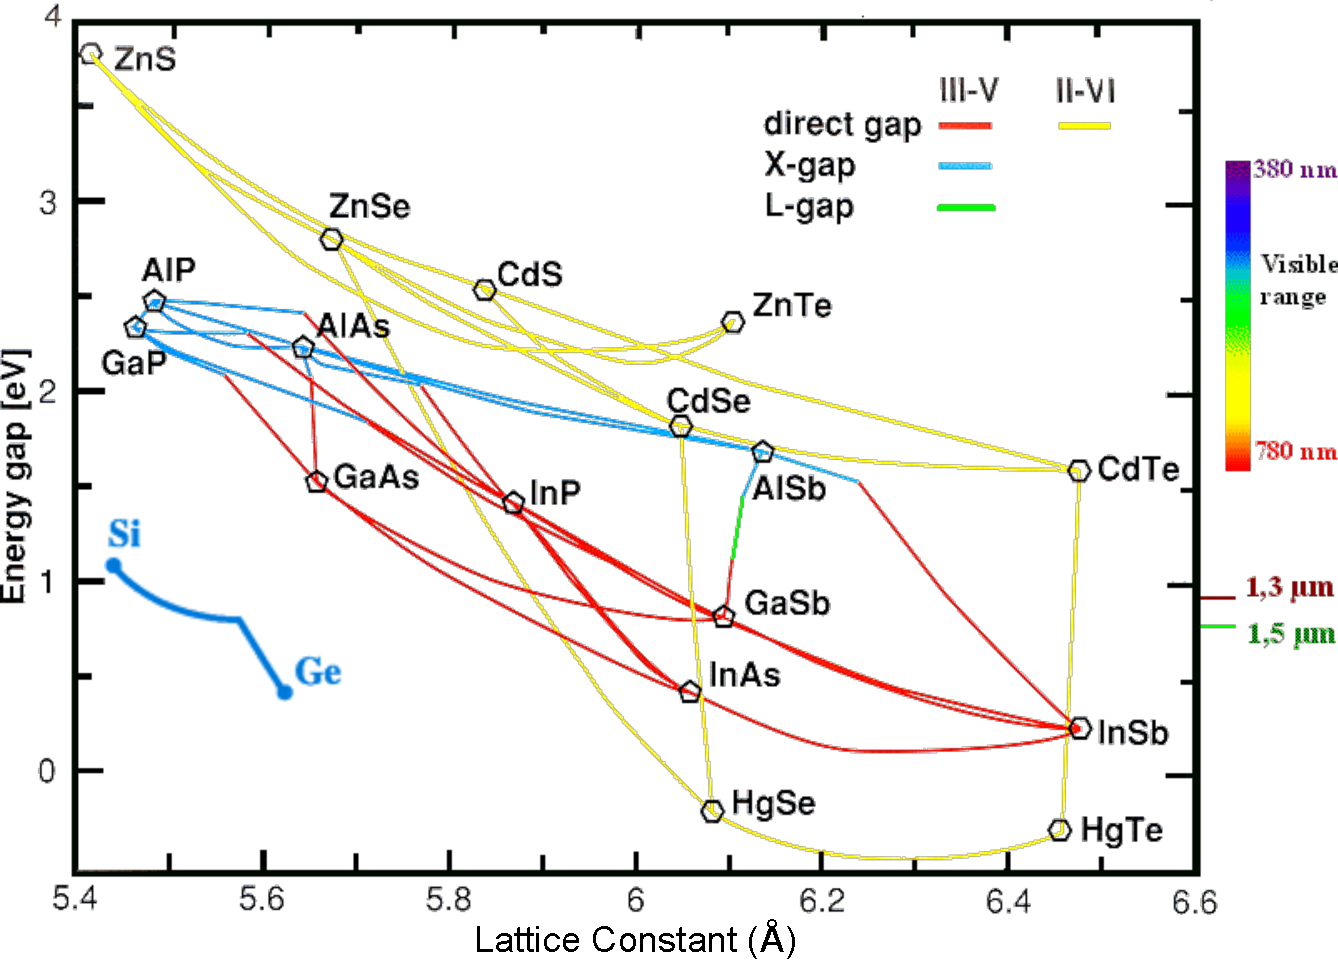
\includegraphics[width=0.9\textwidth]{intro_bandgaps}
 \caption[Bandgap versus lattice constant]{\label{fig:intro_bandgaps}Bandgap versus lattice constant for the most common semiconductors (modified from Helmut\cite{HelmutFoll2013}) (used with permission)}
\end{figure}

Beyond the III-V homologous growth systems, the next most investigated epitaxial process is when these materials are grown on silicon.
In addition to the always-present issue of strain due to the intrinsic lattice mismatch between the III-V family and silicon, the diamond structure of silicon results in an issue of polar (zincblende) on non-polar (diamond) epitaxy\cite{Kroemer1987} where group III and group V atoms cannot differentiate between sites on the silicon surface.
Such site non-specificity has been an issue of great interest to the epitaxy research community resulting in numerous attempts (some successful)\cite{Kroemer1987} to improve growth of such a chemically dissimilar system.

Outside the extensive research into the epitaxy of silicon and the III-V systems, work into epitaxy has mostly been on a material-by-material basis.
Material systems of interest are examined on an issue by issue basis with the goal of producing high quality material for some application, rather than examining the generalized epitaxy phenomenon.
In this work, the goal has been to expand the understanding of epitaxy through an experimental exploration of several model systems which are corner cases of epitaxy, and to show other conditions under which high quality epitaxy can occur.
Through this work, two key themes were examined in epitaxial systems, the role of symmetry and the role of energy at epitaxial interfaces.
These themes were examined through investigations into three model material systems, III-V semiconductors on silicon, II-VI semiconductors on crystalline oxides, and noble metals on crystalline oxides.
Investigations into III-V semiconductors on silicon focused on the role of vicinal surfaces, surface reconstructions, and higher order crystal surfaces.
Vicinal (or offcut) surfaces of substrates, truncated and reconstructed, were found to have a strong effect on twinning during epitaxial growth, a potential method of improving quality of material growth.
(211), a higher order substrate orientation was found to allow accommodation of strain by tilting of a growing epitaxial layer.
Investigations into II-VI semiconductors concentrated on the role of surface reconstructions, and the role of bond strength in epitaxial interfaces.
A new epitaxial relationship between temperature stable surface reconstruction and CdTe was observed and atomically modeled, such stable surface reconstructions may offer a new route for lattice matched epitaxial growth.
In addition, growths of CdTe on sapphire substrates were found to show a unique liftoff phenomenon, where single crystal films are weakly bonded to the substrate and can be removed while maintaining crystalinity.
Finally, investigations into noble metals on oxide surfaces concentrated on the properties of epitaxy in the weak bonding regime.
Epitaxial growth of gold on spinel, a complex oxide, was found to be possible, despite the weak reactivity of both the noble metal and the oxide substrate.
The results from these investigation and the main contribution of this work is to show that epitaxy is possible for symmetrically and chemically dissimilar model systems, and to experimentally examine the implications to epitaxy that such systems have.

\section{Major Themes}
\subsection{Symmetry} The 2D (and as we shall later see sometimes 3D) interface that separates the epitaxial substrate from the growing crystal has a symmetry relationship which relates the substrate to the crystal.
These surface symmetries are different than the bulk symmetry of the substrate and crystal.
In the simplest treatment of surfaces, the surface of a given substrate is simply a truncation of the crystal in a given orientation, exposing a plane of atoms which then present a subsymmetry of the bulk crystal.
Any truncation through a bulk crystal is unstable, since the once buried atoms are now exposed at a surface, this surface can resolve this instability in a variety of ways.
As will be seen later there are many complications to this model and it is in these complications that we find changes in symmetry, breaks in symmetry and distortions of this 2D surface into a more complex 3D interface.
It is these changes to the surface symmetry, and it's interaction with the growing crystal which have profound and useful implications for epitaxy.
The first major theme investigates the implications of unique interface symmetries, broken symmetries and 3D interfaces on the epitaxial process.

\subsection{Energy} While the symmetry of a surface describes the spatial distribution of the potential landscape presented to a growing crystal, energy describes the magnitude that potential landscape has on a growing crystal.
Strong energy landscapes cause the symmetry of a given substrate to have it's influence felt strongly, while a weak landscape can have a subtle effect on growth.
Whether atoms are bonded via physisorption, covalent bonding, ionic attraction or Van der Walls forces determines the strength of the interface landscape energy.
The energy landscape of the epitaxial interface can vary over a large range, and the role of these strengths has not been examined extensively.
The second major theme of this work investigates the implications of energy landscapes outside the typical heteroepitaxy regime, specifically relating to the weaker energies.

\section{Secondary Themes}\todo{Provide clearest example where this is true}
\subsection{Combined Reciprocal Space and Real Space Characterization} The investigations into epitaxy discussed throughout this thesis have relied upon a variety of techniques to reveal the patterns behind these processes.
The most fruitful of the techniques utilized in this work has been the combined use of reciprocal space mapping via 2DXRD and the direct imaging of samples using TEM/STEM\@. These techniques, when used individually, often lead to ambiguity in the results.
STEM/TEM, being a small-area sampling technique can frequently miss information, or cause false interpretations of ``common'' results, when a given sample may be unique or atypical.
Similarly, the use of reciprocal space mapping alone gives a picture which convolves all of the data in the sampling area together, providing little insight about its spatial distribution.
When these two techniques are combined, the two datasets must be successfully reconciled for a given model of the underlying system to be coherent.
Such consistency requirements allow competing explanations to be discriminated from one another based on predictions they make about the data, leading to more complete and less ambiguous models.
Such a combination of techniques has also encouraged collaboration, as one cannot be an expert in the operation and interpretation of both systems without compromising the work one originally intended to do.
